%%%%%%%%%%%%%%%%%%%%%%%%%%%%%%%%%%%%%%%%%
% Introduction
% 
% $Date$
% $Revision$
% $Author$


\chapter{Introduction}

% \TODO{Introductional text}

%%
\section{What is \Kieker?}\label{sec:kieker}

The \Kieker{} framework allows to monitor and to analyze runtime behavior %
of Java applications. Examples of runtime behavior are application-internal %
control flows and response times of method executions. %
% Normal ({}``plain) Java applications can be arranged with the framework as well %
% as server based Java web applications. 
% The framework itself has been developed with regard to providing an easy manageable, %
% maintainable piece of software, which can be included uncomplicated into both, %
% new and existing software projects. 
Kieker has been designed for continuous operation, inducing only a very low %
overhead during the monitoring. 
% Kieker can probe whole method calls as well as single statements (e.g. a = a + 1).\\ 

% This is the component diagram of Kieker (the satellite).
\begin{figure}[H]\centering
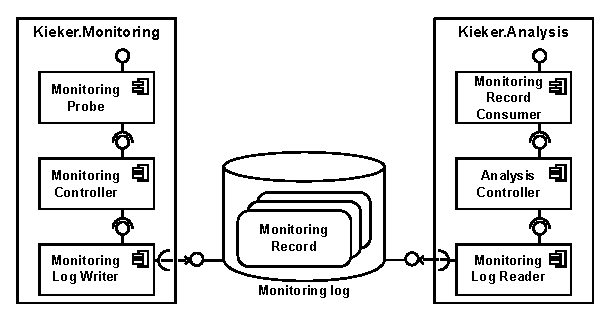
\includegraphics[width=0.73\textwidth]{images/kiekerComponentDiagram-woCloud-bw-w-record-newNames}
\caption{Overview of the framework components}
\label{Figure:KiekerComponentDiagram}
\end{figure}
		
\noindent Figure \ref{Figure:KiekerComponentDiagram} shows that the framework %
is structured into two main components:% \KiekerMonitoringPart{} and \KiekerAnalysisPart{}:
\begin{description}
 % Both items get notify-tags because of the important information in here.
 % avh: Removed them because we shouldn't use them "inflationaryly"
\item[\KiekerMonitoringPart]
is responsible for the program instrumentation, data %
collection and logging. Its core is the class \class{MonitoringController} %
which receives the monitoring data in so-called monitoring records and %
writes these monitoring records into the configured monitoring log---e.g., %
located in a filesystem or in a database.
\item[\KiekerAnalysisPart]
is responsible for the analysis and possible visualization of the %
monitoring data. Its core is the class \class{AnalysisInstance} %
which manages the life-cycle of the monitoring log reader and all analysis plugins.
\end{description}


\noindent Both parts are composed of subcomponents---those included in the %
Kieker distribution and/or custom implementations. The important interaction pattern among %
the components is illustrated in Figure \ref{Figure:KiekerCommunicationDiagram} %
but will be explained furthermore throughout the course of this tutorial. %

% This image shows the communication diagram of the different components.
\begin{figure}[H]\centering
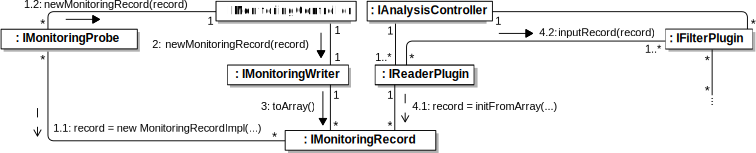
\includegraphics[width=1\textwidth]{images/kiekerCommunications-revisedReArranged-woMonitoringLog-bw-newNames}
\caption{Communication among \Kieker{} framework components}
\label{Figure:KiekerCommunicationDiagram}
\end{figure}
		
% Notify-tag because it is explained how Kieker works.
% avh: removed
\noindent The monitoring probes create the monitoring records included the %
monitoring data and deliver them to the monitoring controller. %
The monitoring controller employs the monitoring log writers to write these %
monitoring records to the monitoring log. %
For analysis, a monitoring log reader reads the records from the monitoring log, 
which are then passed  who creates a monitoring record again. These records can %
then be further processed by the analysis plugins.

%%
% \section{Features}

Kieker includes monitoring log writers and readers for filesystems, SQL %
databases, and the Java Messaging Service~(JMS)~\cite{JMS-WebSite}. %
A special feature of Kieker is the ability to monitor and analyze (distributed) %
traces of method executions and corresponding timing information. %
For this purpose, Kieker includes monitoring probes employing %
AspectJ~\cite{AspectJ-WebSite}, %
Java~EE Servlet~\cite{JavaServletTechnology-WebSite}, %
Spring~\cite{Spring-WebSite}, and %
Apache~CXF~\cite{CXF-WebSite} technology. %
The \KiekerTraceAnalysis{} tool allows to reconstruct and visualize %
architectural models of the monitored systems, e.g., as sequence and %
dependency diagrams.

%%	
\section{Structure of this User Guide}

Based on a simple example, Chapter~\ref{chap:example} demonstrates %
how to manually instrument Java programs with \KiekerMonitoringPart{} %
in order to monitor timing information of method executions, and %
how to use \KiekerAnalysisPart{} to analyze the monitored data. %
Chapter~\ref{chap:componentsMonitoring} provides a more detailed %
description of \KiekerMonitoringPart{} and shows how to implement and %
use custom monitoring records, monitoring probes, and monitoring log writers. %
A more detailed description of \KiekerAnalysisPart{} and how to implement and use %
custom monitoring log readers, and analysis plugins follows in %
Chapter~\ref{chap:componentsAnalysis}. %
Chapter~\ref{chap:aspectJ} demonstrates how to use \KiekerTraceAnalysis{} %
for monitoring and analyzing/visualizing traces. %

\quad\\

% Notify-tag because this could be interesting for the reader.
\NOTIFYBOX{The Java sources presented in this user guide are included in the %
\file{\exampleDirFull/} directory of the \Kieker{} distribution (see %
Section \ref{sec:example:downloadInstall}).}

% \TODO{Point to Web site for additional examples, TR, \ldots}
